\newpage
\section{Durchführung}
\label{sec:Durchfuehrung}
    Die Durchführung des Versuchs ist in drei Teile geteilt, zunächst werden im ersten Teil des Versuches die Moden des verwendeten Hohlleiters untersucht. Im zweiten Teil des Versuches soll die Frequenz, die Wellenlänge und die Dämpfung für die Mikrowellen bestimmt werden. Abschließend werden im letzten Versuchsteil stehende Wellen untersucht.
    \subsection{Versuchsaufbau}
        Um die für den Versuch notwendigen Mikrowellen zu erzeugen wird ein Reflexklystron (\ref{sec:Reflexklystron}) welches mit einer variablen Spannungsquelle versorgt wird verwendet.
        Nach der Mikrowellenquelle wird ein Einweggleichrichter platziert, welcher verhindert dass reflektierte Wellen in das Klystron gelangen.
        Nach dem Einweggleichrichter wird ein Frequenzmesser eingesetzt mit dessen Hilfe die Frequenz der Mikrowellen genauer bestimmt werden kann.
        Der Frequenzmesser besteht aus einem variablen Hohlraum mit dem der verwendete Hohlraumresonator modifiziert werden kann.
        Nach dem Frequenzmesser wird eine variable Dämpfung eingebaut mit der die Mikrowellen abgeschwächt werden können.
        Dieser Aufbau ist der Grundaufbau für die drei Versuchsteile, in den einzelnen Versuchsteilen werden verschiednen Bauteile hinter die Dämpfung eingesetzt um die Messungen durchzuführen.
    \subsection{Untersuchung der Hohlleitermoden}
        Für die erste Messung wird hinter die Dämpfung lediglich ein Detektor angebracht welcher mit einem Oszilloskop verbunden wird.
        Der Detektor besteht dabei aus einer kleinen Nadel die in den Hohlraum ragt und als Dipol durch die Mikrowellen angeregt werden kann.
        \begin{figure}[H]
            \centering
            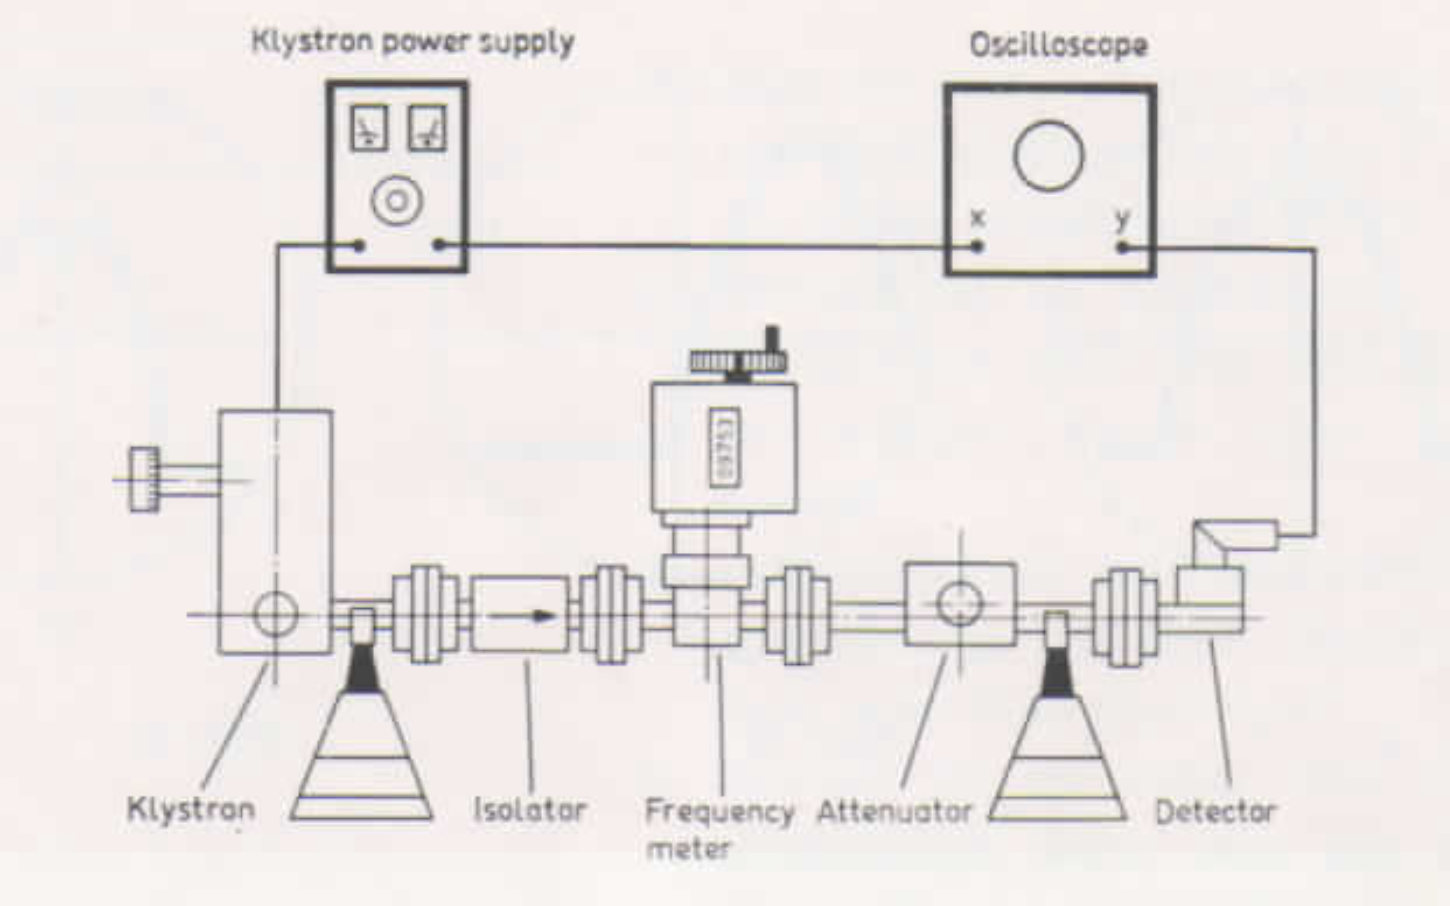
\includegraphics[width = 0.75\textwidth]{bilder/Aufbau_Teil1.png}
            \caption{Aufbau\_Teil1.png}
            \label{fig:Teil1}
        \end{figure}
        Um die Moden des Hohlleiters zu untersuchen wird auf den x-Kanal des Oszilloskops die Betriebsspannung der Reflexklystrons und auf den y-Kanal die Spannung des Detektors gelegt.
        Mit dem Oszilloskop können dadurch die Moden sichtbar gemacht werden (\ref{fig:Moden-Abbildung}).
        \begin{figure}[H]
            \centering
            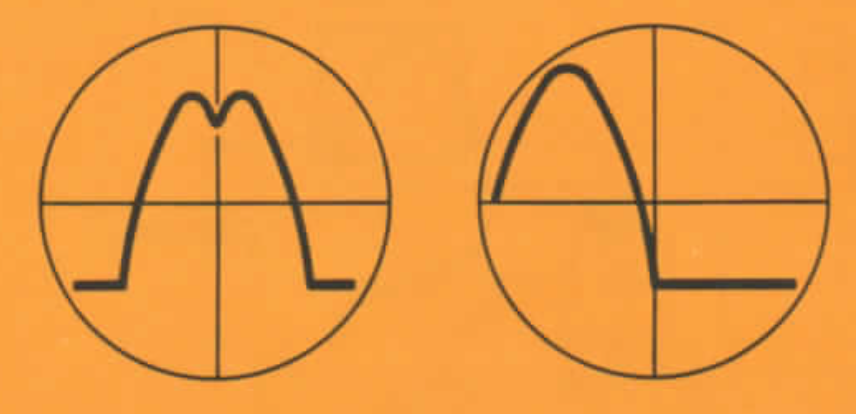
\includegraphics[width = 0.75\textwidth]{bilder/Moden-Abbildung.png}
            \caption{Moden-Abbildung.png}
            \label{fig:Moden-Abbildung}
        \end{figure}
        Die Reflektorspannung wird nun so gewählt, dass die Mitte der Mode mittig auf der x-Achse des Oszilloskops liegt.
        Nun wird der Frequenzmesser eingestellt um die Einbuchtung auf die Mitte der Mode und somit das Maximum zu bewegen und die Mittelfrequenz zu bestimmen.
        Von der Mode werden nun Mittelfrequenz, Reflektorspannung und Amplitude notiert.
        Diese Messung wird für zwei weitere Moden wiederholt und auch notiert.

        Anschließend wird für jede Mode noch die Punkte der halben Leistung vermessen indem jeweils rechts und links neben der Mode die Einbuchtung der Frequenzmessung auf den wert der halben Amplitude gebracht und die Frequenz sowie die Reflektorspannung notiert.
    \subsection{Messung von Frequenz, Wellenlänge und Dämpfung}
        Teil2
        \begin{figure}[H]
            \centering
            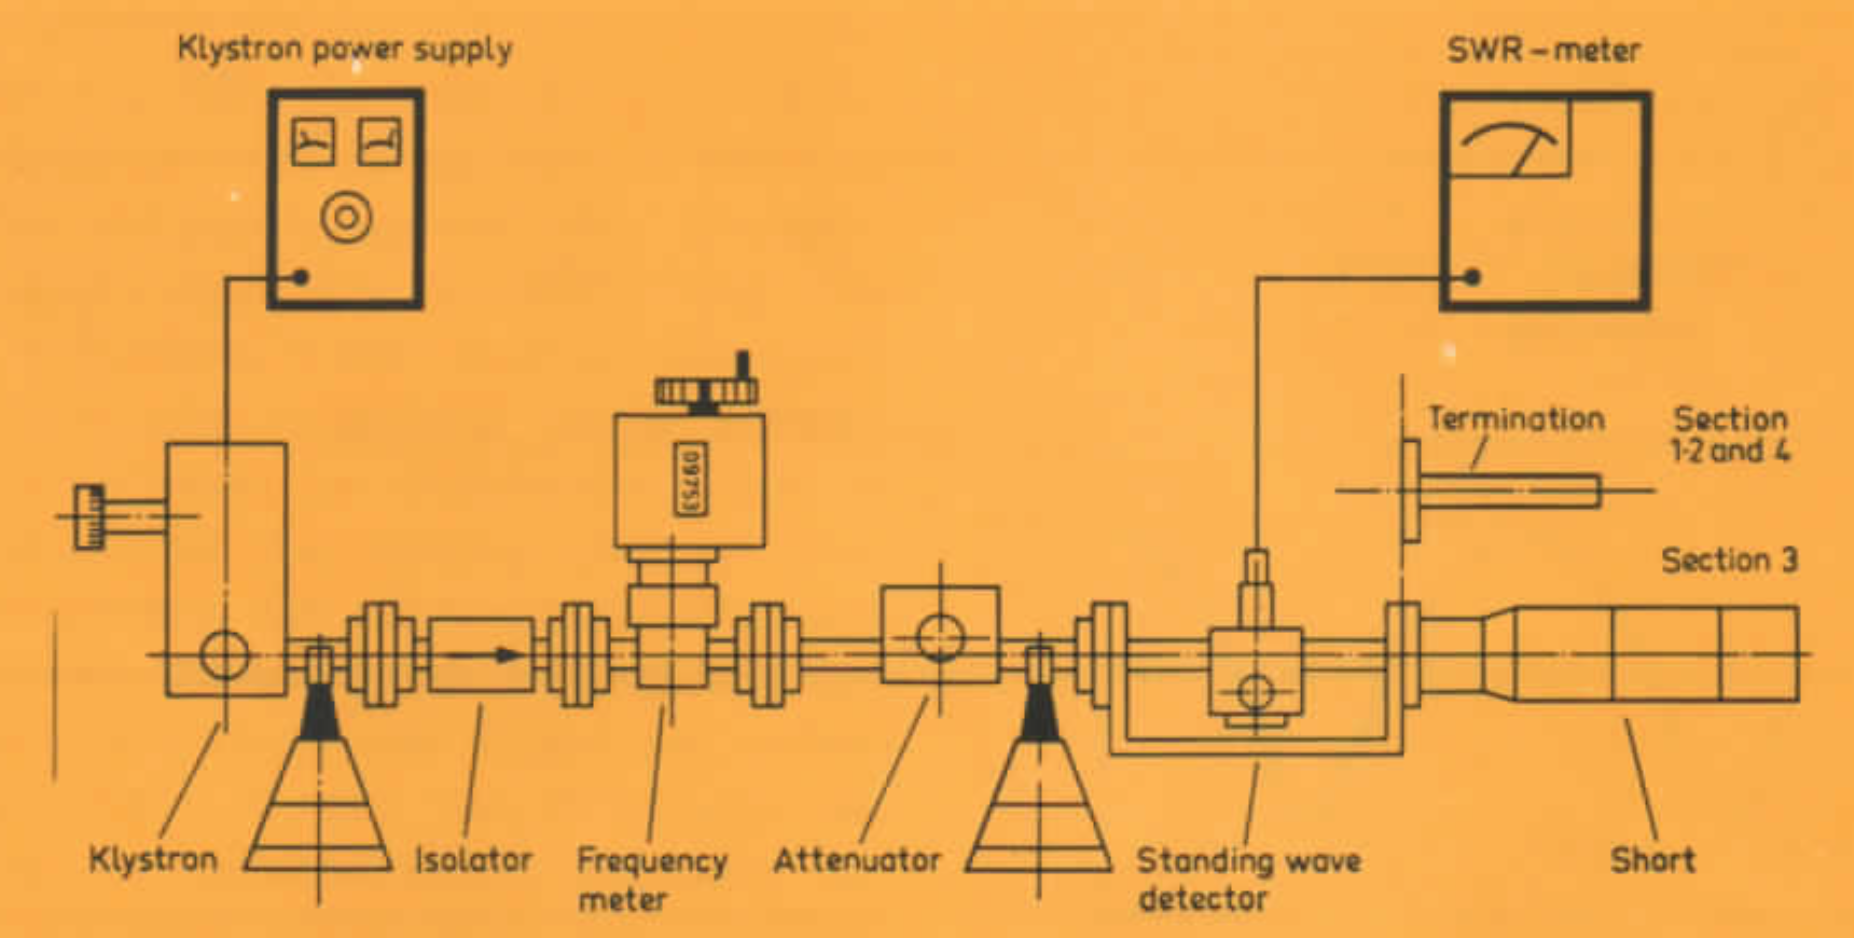
\includegraphics[width = 0.75\textwidth]{bilder/Aufbau_Teil2.png}
            \caption{Aufbau\_Teil2.png}
            \label{fig:Teil2}
        \end{figure}
    \subsection{Untersuchung der Stehenden Wellen}
        Teil3
        \begin{figure}[H]
            \centering
            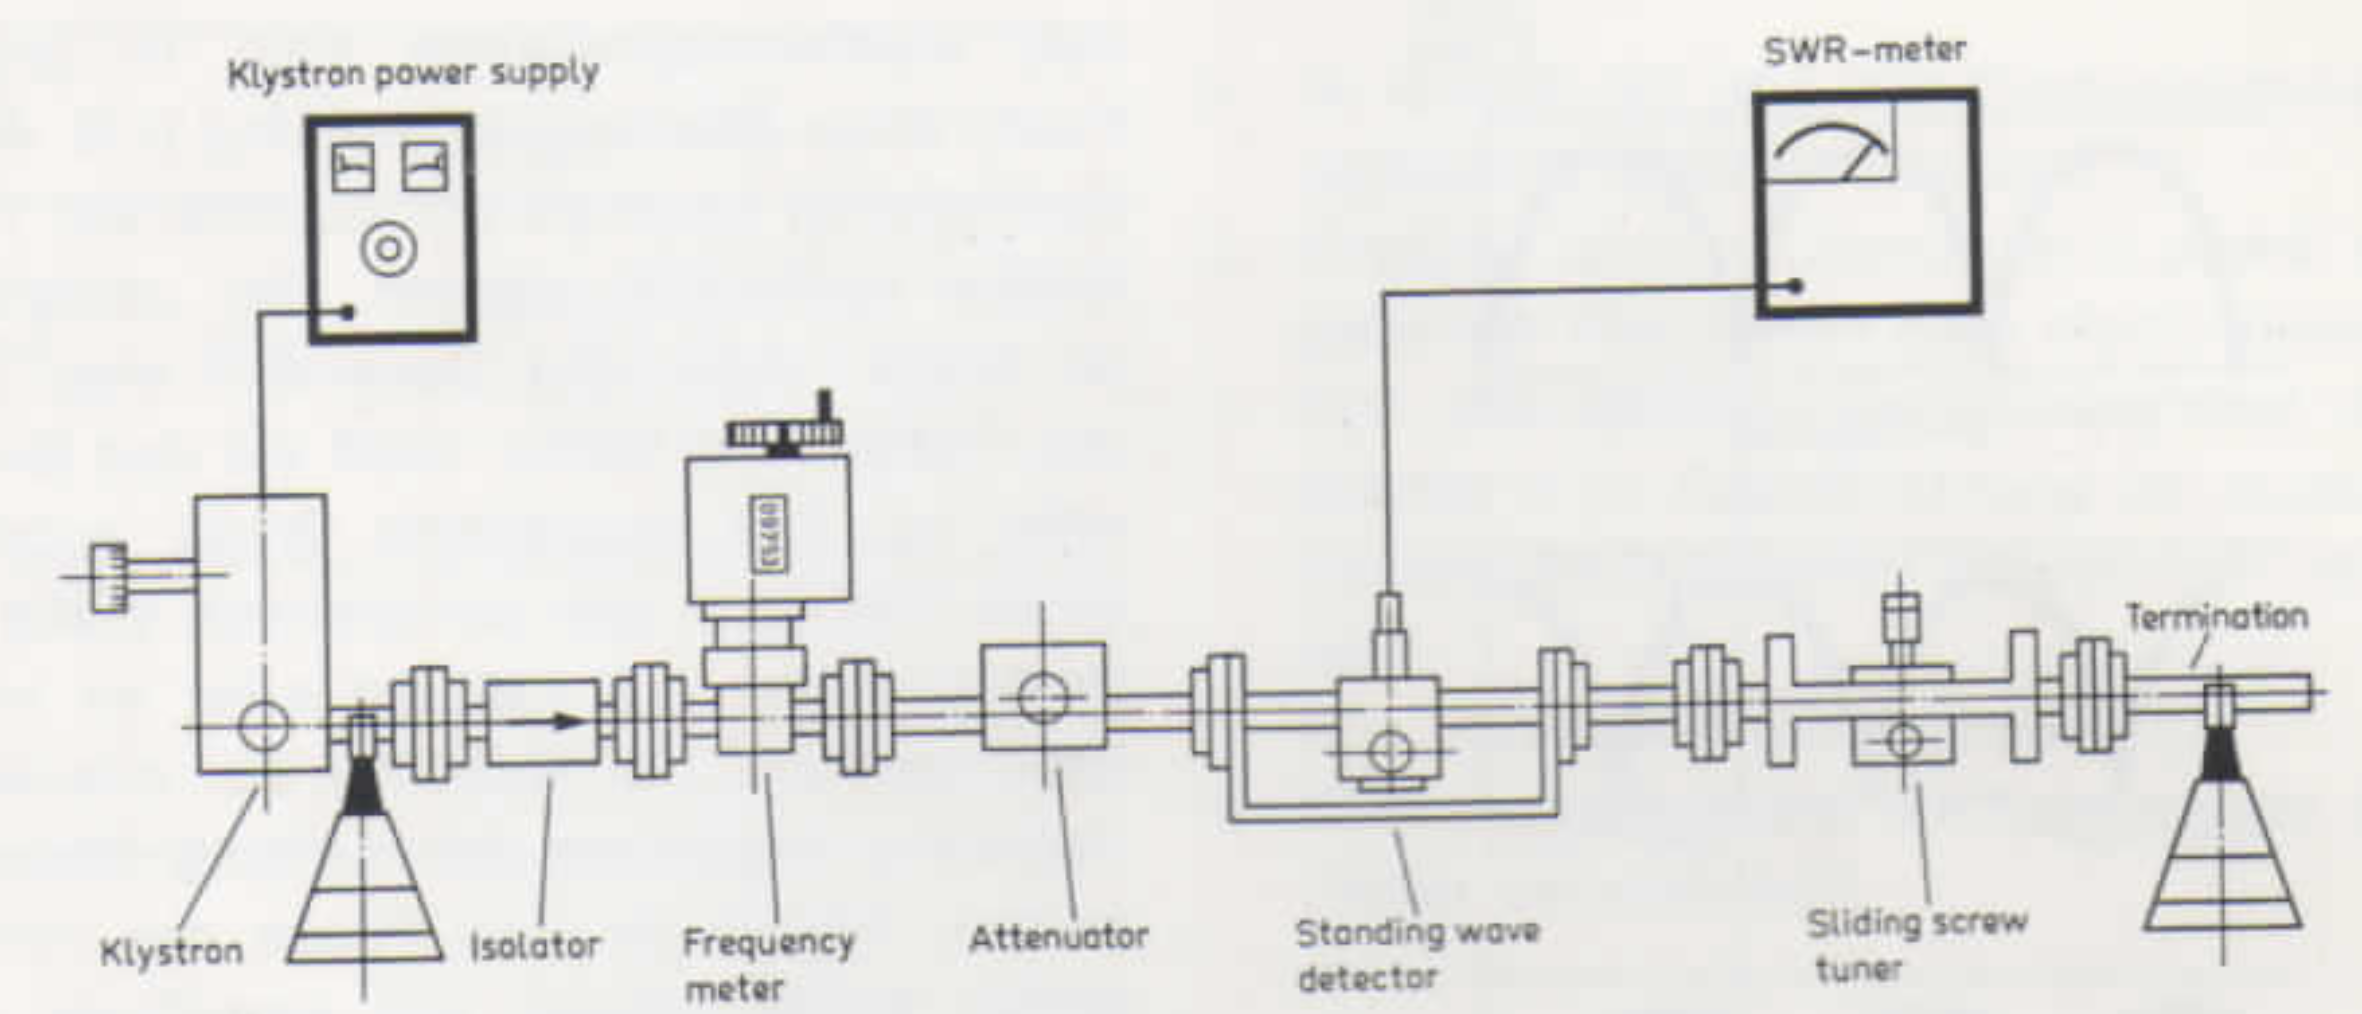
\includegraphics[width = 0.75\textwidth]{bilder/Aufbau_Teil3.png}
            \caption{Aufbau\_Teil3.png}
            \label{fig:Teil3}
        \end{figure}